%		PSAR - Sujet 7
%	INTERFACE GRAPHIQUE POUR LA LOGIQUE
%	Sandra Laduranti et Bastien Rigault
%
%	TeX file pour le cahier des charges

\documentclass{article}

\usepackage[utf8]{inputenc}
\usepackage[T1]{fontenc}
\usepackage[french]{babel}
\usepackage{amsmath, amsthm, amssymb}

\usepackage{amsfonts}
\usepackage{gastex}
\usepackage[dvips]{graphics}
\usepackage{pstricks}
\usepackage{a4wide}
\usepackage{multicol}
\usepackage{pst-tree}
\usepackage{tikz-qtree}


\usepackage{tikz}
\usetikzlibrary{arrows}
\tikzstyle{ent}=[circle,draw,thick,inner sep=0pt,minimum size=2.5mm]
\usetikzlibrary{arrows,automata,positioning}
\usetikzlibrary{automata,patterns,topaths,shapes,calc}
\tikzstyle{every picture}+=[>=stealth',initial text=]
\tikzstyle{state}=[rectangle,draw=black]

\newcommand{\Q}{\mathbb{Q}}
\newcommand{\R}{\mathbb{R}}
\newcommand{\N}{\mathbb{N}}
\newcommand{\Z}{\mathbb{Z}}
\newcommand{\T}{\mathbb{T}}
\newcommand{\Bo}{\mathbb{B}}

\newcommand{\Au}{\mathcal{A}}
\newcommand{\B}{\mathcal{B}}
\newcommand{\C}{\mathcal{C}}
\newcommand{\D}{\mathcal{D}}
\newcommand{\F}{\mathcal{F}}
\newcommand{\G}{\mathcal{G}}
\newcommand{\K}{\mathcal{K}}
\newcommand{\Hr}{\mathcal{H}}
\newcommand{\I}{\mathcal{I}}
\newcommand{\La}{\mathcal{L}}
\newcommand{\M}{\mathcal{M}}
\newcommand{\Net}{\mathcal{N}}
\newcommand{\Pa}{\mathcal{P}}
\newcommand{\Rel}{\mathcal{R}}
\newcommand{\Sy}{\mathcal{S}}
\newcommand{\Ts}{\mathcal{T}}
\newcommand{\X}{\mathcal{X}}

\newcommand{\rel}{\bowtie}
\newcommand{\tr}{\xrightarrow}
\newcommand{\opeq}{\leftrightarrow}
\newcommand{\fee}{\varphi}
\newcommand{\eps}{\varepsilon}
\newcommand{\vect}[1]{\mathbf{#1}}
\newcommand{\fut}{\overrightarrow}
\newcommand\sui[1][a]{\ensuremath{\left(#1_n\right)_{n\in \N}}}

\newcommand{\E}{\textsf{E}}
\newcommand{\A}{\textsf{A}}

\DeclareMathOperator{\cla}{cl}

\theoremstyle{plain}

\newtheorem{theorem}{Théorème}
\newtheorem{lemma}[theorem]{Lemme}
\newtheorem{corollary}[theorem]{Corollaire}
\newtheorem{proposition}[theorem]{Proposition}

\newtheorem{definition}[theorem]{Définition}

\theoremstyle{remark}
\newtheorem{remark}[theorem]{Remarque}
\newtheorem{example}[theorem]{Exemple}

\begin{document}

% PAGE 1
\noindent UPMC, 4I408 \hfill Année 2015--2016 \\
\hfill Sandra Laduranti \\ Bastien Rigault

\begin{center}
	\vspace{4cm}
 	{ \LARGE \bf
 	Projet SAR \\  Une interface graphique pour la logique 
	\\ \vspace{1cm}
 	Cahier des charges
 	}
\end{center}
\clearpage

%PAGE 2
\section{Description du projet}
L'objectif de ce projet, réalisé dans le cadre de l'UE PSAR(4I408) est de concevoir un logiciel pédagogique pour l'apprentissage de la logique du premier ordre. Ce logiciel apportera notamment un support visuel sous la forme d'un jardin et de fleurs permettant d'appréhender plus facilement les formules de la logique. 

\subsection{Logique du premier ordre}
\subsubsection{Les bases de la logique}
La logique du premier ordre enrichit le calcul propositionnel en utilisant :
\begin{itemize}
\item des termes construits avec des variables et des fonctions,
\item des formules construites à partir de relations sur les termes,
  avec des opérateurs booléens et des quantifications sur les
  variables.
\end{itemize}
On note ainsi $F$ l'ensemble de symboles de fonction et $X$ celui des variables (disjoint de $F$). De plus, chaque symbole de $F$ possède une arité définie dans $\N$ qui désigne le nombre d'arguments de la fonction. Ainsi, $F_0$ (l'ensemble des symboles de $F$ d'arité 0) correspond aux constantes (limité à 20 constantes dans notre cas), $F_1$ est l'ensemble des fonctions ayant 1 argument, $F_2$ 2 arguments etc.
\newline
Par exemple on peut écrire la formule suivante :
\begin{center}
$ \forall x \exists y f(x,y) $
\end{center}
Où $\forall$ et $\exists$ sont des quantificateurs, $x$ et $y$ des variables et $f(x,y)$ une fonction d'arité 2. Si $x$ et $y$ sont respectivement des tulipes et des roses et $f(x,y)$ est une relation de taille tel que $x$ est plus petit que $y$ alors on obtient : \textit{Pour toute tulipe $x$ il existe une rose $y$ plus grande qu'elle.}


\subsubsection{Syntaxe}
On définit une formules comme étant un ensemble de termes (fonctions, variables) et de quantificateurs ($\forall$, $\exists$) correctement assemblés.
\newline
Ainsi des formules comme : 
\begin{center}
$\forall \exists x,y f(x,y)$ ou $z f(x,y) \forall$ 
\end{center}
devront être considérés comme des formules syntaxiquement invalides et refusées par le vérificateur syntaxique de formule.
\newline

Par ailleurs on imposera certaines limite au nombre de constante, de variable et de prédicat disponible dans le cadre de ce projet. Ainsi une formule syntaxiquement correct ne devra comprendre que des symboles parmis les ensembles suivants:
\begin{itemize}
	\item L'ensemble $F_0$ limité à 20 constantes ($a, b, ..., t$),
	\item L'ensemble $X$ restreint à 5 variables ($v, w, x, y, z$),
	\item Les ensembles $F_1$ et $F_2$ correspondant aux ensemble des prédicat implentés nativement dans le vérificateur de formule qui seront définis ci-après.
	\item L'ensemble des quantificateurs contenant 2 symboles ($\forall$ et $\exists$)
\end{itemize}
\vspace{0.3cm}
Les prédicats peuvent être divisés en deux catégories :
\begin{description}
	\item \textbf{Les connecteurs logique réservés} à savoir $\lnot$ (negation), $\land$ (et), $\lor$ (ou) et $\Rightarrow$ (implique) qui sont tous binaire.
	\item \textbf{Les prédicats propre au projet} que l'on regroupera par arité :
		\begin{itemize}
			\item[\textit{Unaire}] définissant l'état d'une fleur, elle peut être :
				\begin{itemize}
					\item une rose, une paquette ou une tulipe
					\item petite, moyenne ou grande
					\item rouge, rose ou blanche
					\item à l'est, à l'ouest, au sud ou au nord
				\end{itemize}
			\item[\textit{Binaire}] définissant une relation entre 2 fleurs, la fleur $A$ peut être :
				\begin{itemize}
					\item à l'est, à l'ouest, au sud ou au nord de la fleur $B$
					\item à la même latitude ou longitude que la fleur $B$
					\item plus grande, plus petite ou de même taille que la fleur $B$
					\item de la même couleur que la fleur $B$
				\end{itemize}
			\item[\textit{Ternaire}] définissant une relation entre 3 fleurs, la fleur $C$ peut être :
				\begin{itemize}
					\item Entre la fleur $A$ et la fleur $B$
				\end{itemize}
		\end{itemize}
\end{description}

\subsection{Exemple}

On peut par exemple écrire les huit formules ci-dessous.
\begin{itemize}
    \item [(f1)] $d$ est une rose : Rose($d$)
    \item [(f2)] Toutes les fleurs sont des roses : $\forall x Rose(x)$
    \item [(f3)] Il existe une rose : $\exists x Rose(x)$
    \item [(f4)] Toute fleur blanche est plus petite qu'une fleur située à son est \\
$\forall x (est\_blanc(x) \Rightarrow \exists y  (plus\_petit\_que(x, y) \wedge a\_l\_est\_de(y, x)))$
    \item [(f5)] Toute fleur est à l'est, ou à l'ouest, ou au sud, ou au nord : \\
$\forall x (a\_l\_est(x) \vee a\_l\_ouest(x) \vee au\_sud(x) \vee au\_nord(x))$
    \item [(f6)] Toutes les grandes fleurs sont rouges et il n'existe pas de fleur blanche au sud d'une fleur rouge : \\
    $\forall x (est\_grand(x) \Rightarrow est\_rouge(x))\, \wedge \,\neg \exists x (est\_blanc(x) \wedge \exists y (est rouge(y) \wedge au sud de(x, y)))$
    \item [(f7)] Il existe une fleur rouge au nord de la fleur $g : \exists x (est\_rouge(x) \wedge au nord de(x, g))$
    \item [(f8)] Il existe une unique rose rouge : \\
    $\exists x ((Rose(x) \wedge est rouge(x)) \wedge (\forall y (Rose(y) \wedge est rouge(y)) \Rightarrow x \circeq y))$
\end{itemize}

\clearpage

\section{Fonctionnalités principales}
\subsection{Le jardin}
\begin{figure}[!h]
\begin{center}
\begin{tikzpicture}[scale=0.375]
\node (n0)    at (-9.5,0)      {Ouest};
\node (n0)    at (9,0)      {Est};
\node (n0)    at (0,-9)      {Sud};
\node (n0)    at (0,9)      {Nord};

\node (n0)    at (0,1)      {$\bullet$};
\node (n0)    at (0,3)      {$\bullet$};
\node (n0)    at (0,5)      {$\bullet$};
\node (n0)    at (0,7)      {$\bullet$};
\node (n0)    at (0,-1)      {$\bullet$};
\node (n0)    at (0,-3)      {$\bullet$};
\node (n0)    at (0,-5)      {$\bullet$};
\node (n0)    at (0,-7)      {$\bullet$};

\node (n0)    at (1,0)      {$\bullet$};
\node (n0)    at (3,0)      {$\bullet$};
\node (n0)    at (5,0)      {$\bullet$};
\node (n0)    at (7,0)      {$\bullet$};
\node (n0)    at (-1,0)      {$\bullet$};
\node (n0)    at (-3,0)      {$\bullet$};
\node (n0)    at (-5,0)      {$\bullet$};
\node (n0)    at (-7,0)      {$\bullet$};

\node (n0)    at (1,2)      {$\bullet$};
\node (n0)    at (1,4)      {$\bullet$};
\node (n0)    at (1,6)      {$\bullet$};
\node (n0)    at (1,-2)      {$\bullet$};
\node (n0)    at (1,-4)      {$\bullet$};
\node (n0)    at (1,-6)      {$\bullet$};
\node (n0)    at (-1,2)      {$\bullet$};
\node (n0)    at (-1,4)      {$\bullet$};
\node (n0)    at (-1,6)      {$\bullet$};
\node (n0)    at (-1,-2)      {$\bullet$};
\node (n0)    at (-1,-4)      {$\bullet$};
\node (n0)    at (-1,-6)      {$\bullet$};

\node (n0)    at (2,1)      {$\bullet$};
\node (n0)    at (2,3)      {$\bullet$};
\node (n0)    at (2,5)      {$\bullet$};
\node (n0)    at (2,-1)      {$\bullet$};
\node (n0)    at (2,-3)      {$\bullet$};
\node (n0)    at (2,-5)      {$\bullet$};
\node (n0)    at (-2,1)      {$\bullet$};
\node (n0)    at (-2,3)      {$\bullet$};
\node (n0)    at (-2,5)      {$\bullet$};
\node (n0)    at (-2,-1)      {$\bullet$};
\node (n0)    at (-2,-3)      {$\bullet$};
\node (n0)    at (-2,-5)      {$\bullet$};

\node (n0)    at (3,0)      {$\bullet$};
\node (n0)    at (3,2)      {$\bullet$};
\node (n0)    at (3,4)      {$\bullet$};
\node (n0)    at (3,-2)      {$\bullet$};
\node (n0)    at (3,-4)      {$\bullet$};
\node (n0)    at (-3,0)      {$\bullet$};
\node (n0)    at (-3,2)      {$\bullet$};
\node (n0)    at (-3,4)      {$\bullet$};
\node (n0)    at (-3,-2)      {$\bullet$};
\node (n0)    at (-3,-4)      {$\bullet$};

\node (n0)    at (4,1)      {$\bullet$};
\node (n0)    at (4,3)      {$\bullet$};
\node (n0)    at (4,-1)      {$\bullet$};
\node (n0)    at (4,-3)      {$\bullet$};
\node (n0)    at (-4,1)      {$\bullet$};
\node (n0)    at (-4,3)      {$\bullet$};
\node (n0)    at (-4,-1)      {$\bullet$};
\node (n0)    at (-4,-3)      {$\bullet$};

\node (n0)    at (5,0)      {$\bullet$};
\node (n0)    at (5,2)      {$\bullet$};
\node (n0)    at (5,-2)      {$\bullet$};
\node (n0)    at (-5,0)      {$\bullet$};
\node (n0)    at (-5,2)      {$\bullet$};
\node (n0)    at (-5,-2)      {$\bullet$};

\node (n0)    at (6,1)      {$\bullet$};
\node (n0)    at (-6,1)      {$\bullet$};
\node (n0)    at (6,-1)      {$\bullet$};
\node (n0)    at (-6,-1)      {$\bullet$};

%\draw[dotted] (-8,8) --  (-8,-8);
\draw[dotted] (-7,8) --  (-7,-8);
\draw[dotted] (-6,8) --  (-6,-8);
\draw[dotted] (-5,8) --  (-5,-8);
\draw[dotted] (-4,8) --  (-4,-8);
\draw[dotted] (-3,8) --  (-3,-8);
\draw[dotted] (-2,8) --  (-2,-8);
\draw[dotted] (-1,8) --  (-1,-8);
\draw[->] (0,-8) --  (0,8);
\draw[dotted] (1,8) --  (1,-8);
\draw[dotted] (2,8) --  (2,-8);
\draw[dotted] (3,8) --  (3,-8);
\draw[dotted] (4,8) --  (4,-8);
\draw[dotted] (5,8) --  (5,-8);
\draw[dotted] (6,8) --  (6,-8);
\draw[dotted] (7,8) --  (7,-8);
%\draw[dotted] (8,8) --  (8,-8);

%\draw[dotted] (-8,8) --  (8,8);
\draw[dotted] (-8,7) --  (8,7);
\draw[dotted] (-8,6) --  (8,6);
\draw[dotted] (-8,5) --  (8,5);
\draw[dotted] (-8,4) --  (8,4);
\draw[dotted] (-8,3) --  (8,3);
\draw[dotted] (-8,2) --  (8,2);
\draw[dotted] (-8,1) --  (8,1);
\draw[->] (-8,0) --  (8,0);
\draw[dotted] (-8,-1) --  (8,-1);
\draw[dotted] (-8,-2) --  (8,-2);
\draw[dotted] (-8,-3) --  (8,-3);
\draw[dotted] (-8,-4) --  (8,-4);
\draw[dotted] (-8,-5) --  (8,-5);
\draw[dotted] (-8,-6) --  (8,-6);
\draw[dotted] (-8,-7) --  (8,-7);
%\draw[dotted] (-8,-8) --  (8,-8);

\draw[densely dashed] (0,0) -- (7,7);
\draw[densely dashed] (0,0) -- (-7,-7);
\draw[densely dashed] (0,0) -- (7,-7);
\draw[densely dashed] (0,0) -- (-7,7);
\end{tikzpicture}
\end{center}
\caption{Places d'un jardin}\label{lagrille}
\end{figure}

Les termes considérés dans le projet désignent des fleurs positionnées sur une grille. La figure 1 représente la grille : les points noirs symbolisent les places où peuvent être disposées les fleurs (il y a au plus une fleur par place). Chaque place est identifiée par ses coordonnées (le point $(0,0)$ est au centre de la grille). L'ensemble des places possibles est donc :

\[
\mathrm{Places}  = \left \{
\begin{array}{c}
(0,7) ,
\\
(-1,6), (1,6) ,
\\
(-2,5) , (0,5) , (2,5),
\\
(-3,4) , (-1,4) , (1,4) , (3,4),
\\
(-4,3), (-2,3), (0,3) , (2,3), (4,3),
\\
(-5,2),(-3,2) , (-1,2) , (1,2) , (3,2), (5,2),
\\
(-6,1),(-4,1), (-2,1), (0,1) , (2,1) , (4,1),(6,1),
\\
(-7,0) , (-5,0) , (-3,0) , (-1,0) , (1,0) , (3,0) , (5,0) , (7,0) ,
\\
(-6,-1),(-4,-1), (-2,-1), (0,-1) , (2,-1), (4,-1),(6,-1),
\\
(-5,-2),(-3,-2), (-1,-2), (1,-2) , (3,-2),(5,-2),
\\
(-4,-3), (-2,-3) , (0,-3) , (2,-3), (4,-3),
\\
(-3,-4), (-1,-4), (1,-4) , (3,-4) ,
\\
(-2,-5) , (0,-5) , (2,-5),
\\
(-1,-6),  (1,-6),
\\
(0,-7)
\\
\end{array}
\right \}
\]

Chaque fleur appartient à une espèce (les roses, les pâquerettes et les tulipes), est d'une certaine taille(grande, moyenne ou petite) et d'une certaine couleur (rouge, rose, blanche).

 \begin{center}
 $Especes = \left \{rose, paquerette,tulipe\right \} \, Tailles = \left \{grand, moyen, petit\right \} \, Couleurs = \left \{rouge,rose, blanc\right \}$
 \end{center}

Certaines fleurs ont un nom : il s'agit d'une constante de $F_0$ (deux fleurs différentes ne peuvent pas avoir le même nom). Un jardin $j$ est la donnée d'une grille sur laquelle sont disposées des fleurs (chaque jardin contient
au moins une fleur) et est représentée par une liste de quintuplets. Chaque quintuplet $((x, y), e, t, c, n) \in j$ est un  élément du produit cartésien :

 \begin{center}
 $Places \times Especes \times Tailles \times Couleurs \times(F_0 \cup \left \{None\right \})$ 
 \end{center}
 
\noindent
et exprime qu'une fleur de nom $n$ ($n$ = None si la fleur n'a pas de nom), d'espèce $e$, de taille $t$ et de couleur $c$ se trouve à la place $(x, y)$ dans le jardin j. L'ensemble des jardins possibles est donc :
 
  \begin{center}
  $J = \wp(Places \times Especes \times Tailles \times Couleurs \times(F_0 \cup \left \{None\right \})\setminus\left \{\emptyset\right \}$ 
 \end{center}
 
\subsection{Exemples de formules}

TODO: A REMPLIR AVEC DIVERS EXEMPLES

\clearpage
\subsection{Aspect graphique}
\subsubsection{En résumé}
\begin{itemize}
	\item Un jardin représenté par une grille de taille fixe.
	\item Des fleurs pouvant être disposées sur le jardin et ayant un visuel différent selon leurs espèces, tailles et couleurs.
	\item Un menu permettant de positionner de nouvelles fleurs à la souris et d'en changer leurs aspect.
	\item Un menu permettant d'écrire et vérifier des formules de la logique du premier ordre à l'aide d'un clavier virtuel et d'une liste de 5 variables et 20 constantes.
	\item Un menu permettant de sélectionner une variable ou une constante.
	\item Un clavier visuel permettant de sélectionner les fonctions de la logique (not, et, ou, pour tout etc).
	\item Un menu permettant de sauvegarder et charger des jardins et/ou des ensemble de formules.
\end{itemize}

\subsubsection{Simulation de rendu}

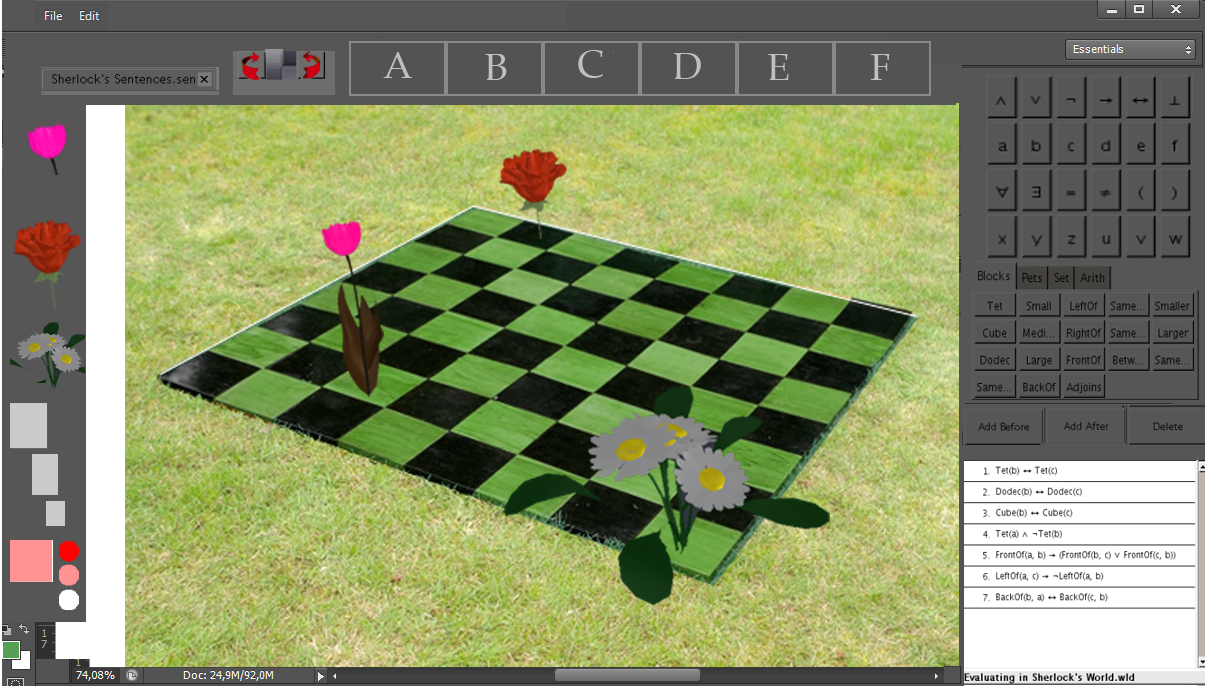
\includegraphics{simulation} ;

\section{Aspect technique}
\subsection{Analyse syntaxique}

\medskip \noindent \textbf{Analyse lexicale :} première étape, découpe la formule en petites entités: opérateurs, mots réservés, variables, constantes, etc.
\medskip \noindent \textbf{Analyse Syntaxique :} seconde étape, explicite la structure de la formule sous forme d'un arbre appelé arbre de syntaxe. Chaque noeud de cet arbre correspond à un opérateur et ses fils aux opérandes sur lesquels il agit.

\begin{figure}[!h]
\begin{center}
\Tree [.S [.NP [.Det Toutes ] [.N les ] ]
[.NP [.N fleurs ]
[.VP [.V sont ]
[.NP [.Det des ] [.N roses ] ] ] ] ]
\caption{Arbre syntaxique}\label{arbresyntaxique}
\end{center}
\end{figure}

\noindent Lors de la vérification de la syntaxe de la formule, le programme stoppera immédiatement l'analyse syntaxique à la première erreur rencontrée. Il informera l'étudiant de la non respect de la syntaxe sur sa formule.

Si l'analyse syntaxique passe tous les tests, la formule sera alors envoyé au au moteur logique pour vérification de sa conformité dans l'environnement donné.

\subsection{Interprétation des formules}
L'interprétation des formules sera réalisée en trois parties distinctes, à savoir leur récupération, la vérification de leur intégrité syntaxique (vue au chapitre précédent) et enfin la vérification de leur validité dans le jardin donné.

\subsubsection{Choix des langages}
Le choix des langages a été régit par la contrainte de communication entre deux langages de programmation différents. L'outil de vérification de formules fourni de base étant en Ocaml, le besoin premier était de trouver comment communiquer avec ce dernier. 
En parallèle il fallait prendre également prendre en compte les contraintes esthétiques, l'application devant être au final à la fois solide et conviviale, la solution de la programmation en Java a donc été immédiatement éliminée par soucis de manque d'esthétisme dans ses GUI.

Suite à de nombreuses recherches, le choix s'est donc porté sur du C\#, offrant un outil de développement permettant de faire le pont entre Ocaml et C\#.
De plus le choix de C\# a été confortée par la possibilité d'utiliser ce langage avec le moteur de jeu Unity 5. 
Les avantages de ce moteur étant tout d'abord sa gratuité mais également son moteur 3D qui entre en parfaite adéquation avec les objectifs finaux du projet.

\subsubsection{Interprétation des formules}
En premier lieu, l'étudiant entrera dans l'application , à l'aide de sa souris et sur le clavier optique fourni par le programme, une formule à valider.
La formule sera alors récupérée via les événements de la GUI de Unity et seront alors transmis à la partie analyse syntaxique de l'application via C\# (vue au chapitre de l'analyse syntaxique). En supposant que la formule ait passé la vérification, elle sera alors envoyé au vérificateur de formule.

Comme vu précédemment, cette partie a impliqué le choix du langage de par sa complexité en terme de programmation. Peu de langages permettent de faire la liaison avec Ocaml. Les formules récupérées préalablement en C\# seront donc transmises via un "pont" formé par l'outil CSML. Cette étape nécessite de renvoyer également le jardin dans son nouvel état, des modifications pouvant être apportées entre deux formules.

Le vérificateur de formule en Ocaml pourra ensuite vérifier l'exactitude de la formule dans le contexte donné et de renvoyer le résultat via le pont CSML à l'application en C\# qui remontera alors graphiquement à l'étudiant la décision de l'application.


\section{Organisation}
\subsection{Outils}
Il a été décidé d'utiliser un gestionnaire de version pour faciliter l'accès aux documents et le travail en parallèle via des branches de développement.
Le choix s'est porté sur github qui offre des repos privés aux étudiants.

\subsection{Partage des tâches}
TODO: a remplir

\section{Fonctionnalités optionnelles}
\subsection{Aspect graphique}
\begin{itemize}
	\item Animation lors de l'ajout d'une fleur et/ou temps d'inactivité de l'utilisateur trop long.
	\item Rendre la saisie de formule possible au clavier uniquement avec un système de raccourci.
\end{itemize}
\subsection{Aspect technique}
\begin{itemize}
	\item Améliorer l'algorithme de vérification syntaxique des formules pour indiquer ou se trouve l'erreur.
	\item Implémenter un système de "retour en arrière"
\end{itemize}
\subsection{Autres idées}
Créer une base de donnée d'exercice permettant à l'étudiant de s'évaluer seul au travers d'un système proposant des problèmes successif aboutissant à une note.

\end{document}
